
% Four-point D3-PA comparison: retain the author-supplied comparison data.
% Reference digitisation and comparison/numerical-verification checks remain
% distinct from the reported arithmetic agreement; do not infer a new area basis.
\subsection{Validation benchmark}
\label{sec:du-validation}

\noindent\textbf{Four-point experimental comparison.} The independent heat-transfer benchmark uses the D3 projected-area (PA) experimental series of \citet{du2025}. Four Nusselt numbers obtained with the present quasi-periodic inlet--outlet loop are compared with the experimental reference over the reported range $2089.966\leq\mathrm{Re}\leq6597.217$. This separate benchmark is not an additional member of the 29-case parameter matrix. Table~\ref{tab:du-validation-comparison} records the four numerical results, the corresponding supplied reference digitisation and the reported signed differences, providing a multi-point assessment of the predicted D3 heat-transfer response.

\paragraph{Experimental benchmark and data provenance.}
Du et al. report a D3 pressing depth of 2.0~mm, dimple pitch of 7.6~mm and dimple size of 2.0~mm, with a $90\degree$ layout and 0.25~mm plate thickness (their Table~3). The water--water experiment used vertical counterflow with cold- and hot-side inlet temperatures of 50 and 70~$^\circ$C, respectively. The selected reference is the \emph{open blue triangle} D3-PA series in their Figure~4(b), not the filled D3 effective-area (EA) markers, their fitted correlation, or their separate D1 numerical-validation results. PA and EA denote two area-based reductions of the same D3 experiment, not different dimple geometries. The supplied reference points are digitised graph estimates rather than a published numerical data table. The comparisons below use the reference values reported in Table~\ref{tab:du-validation-comparison}.

Figure~\ref{fig:du-d3-geometry} shows the reconstructed D3 unit-cell fluid domain used for the benchmark, with its principal dimensions listed in Table~\ref{tab:du-d3-dimensions}. The supplied CAD has opposing cut planes separated by 7.60~mm in both in-plane directions and a nominal 2.00~mm central contact footprint. Its approximately 4.00~mm full vertical envelope describes both bounding walls and must not be interpreted as a uniform local channel gap or as the plate thickness. The 0.25~mm experimental plate thickness is reported for provenance only; no solid plate volume is included in this fluid-domain geometry.

% Dimensioned D3 geometry from the supplied, unmodified fluid-domain STEP.
% Panel arrangement and dimension table remain editable LaTeX.
\begin{figure}[H]
  \centering
  \begin{minipage}[t]{0.49\linewidth}
    \centering
    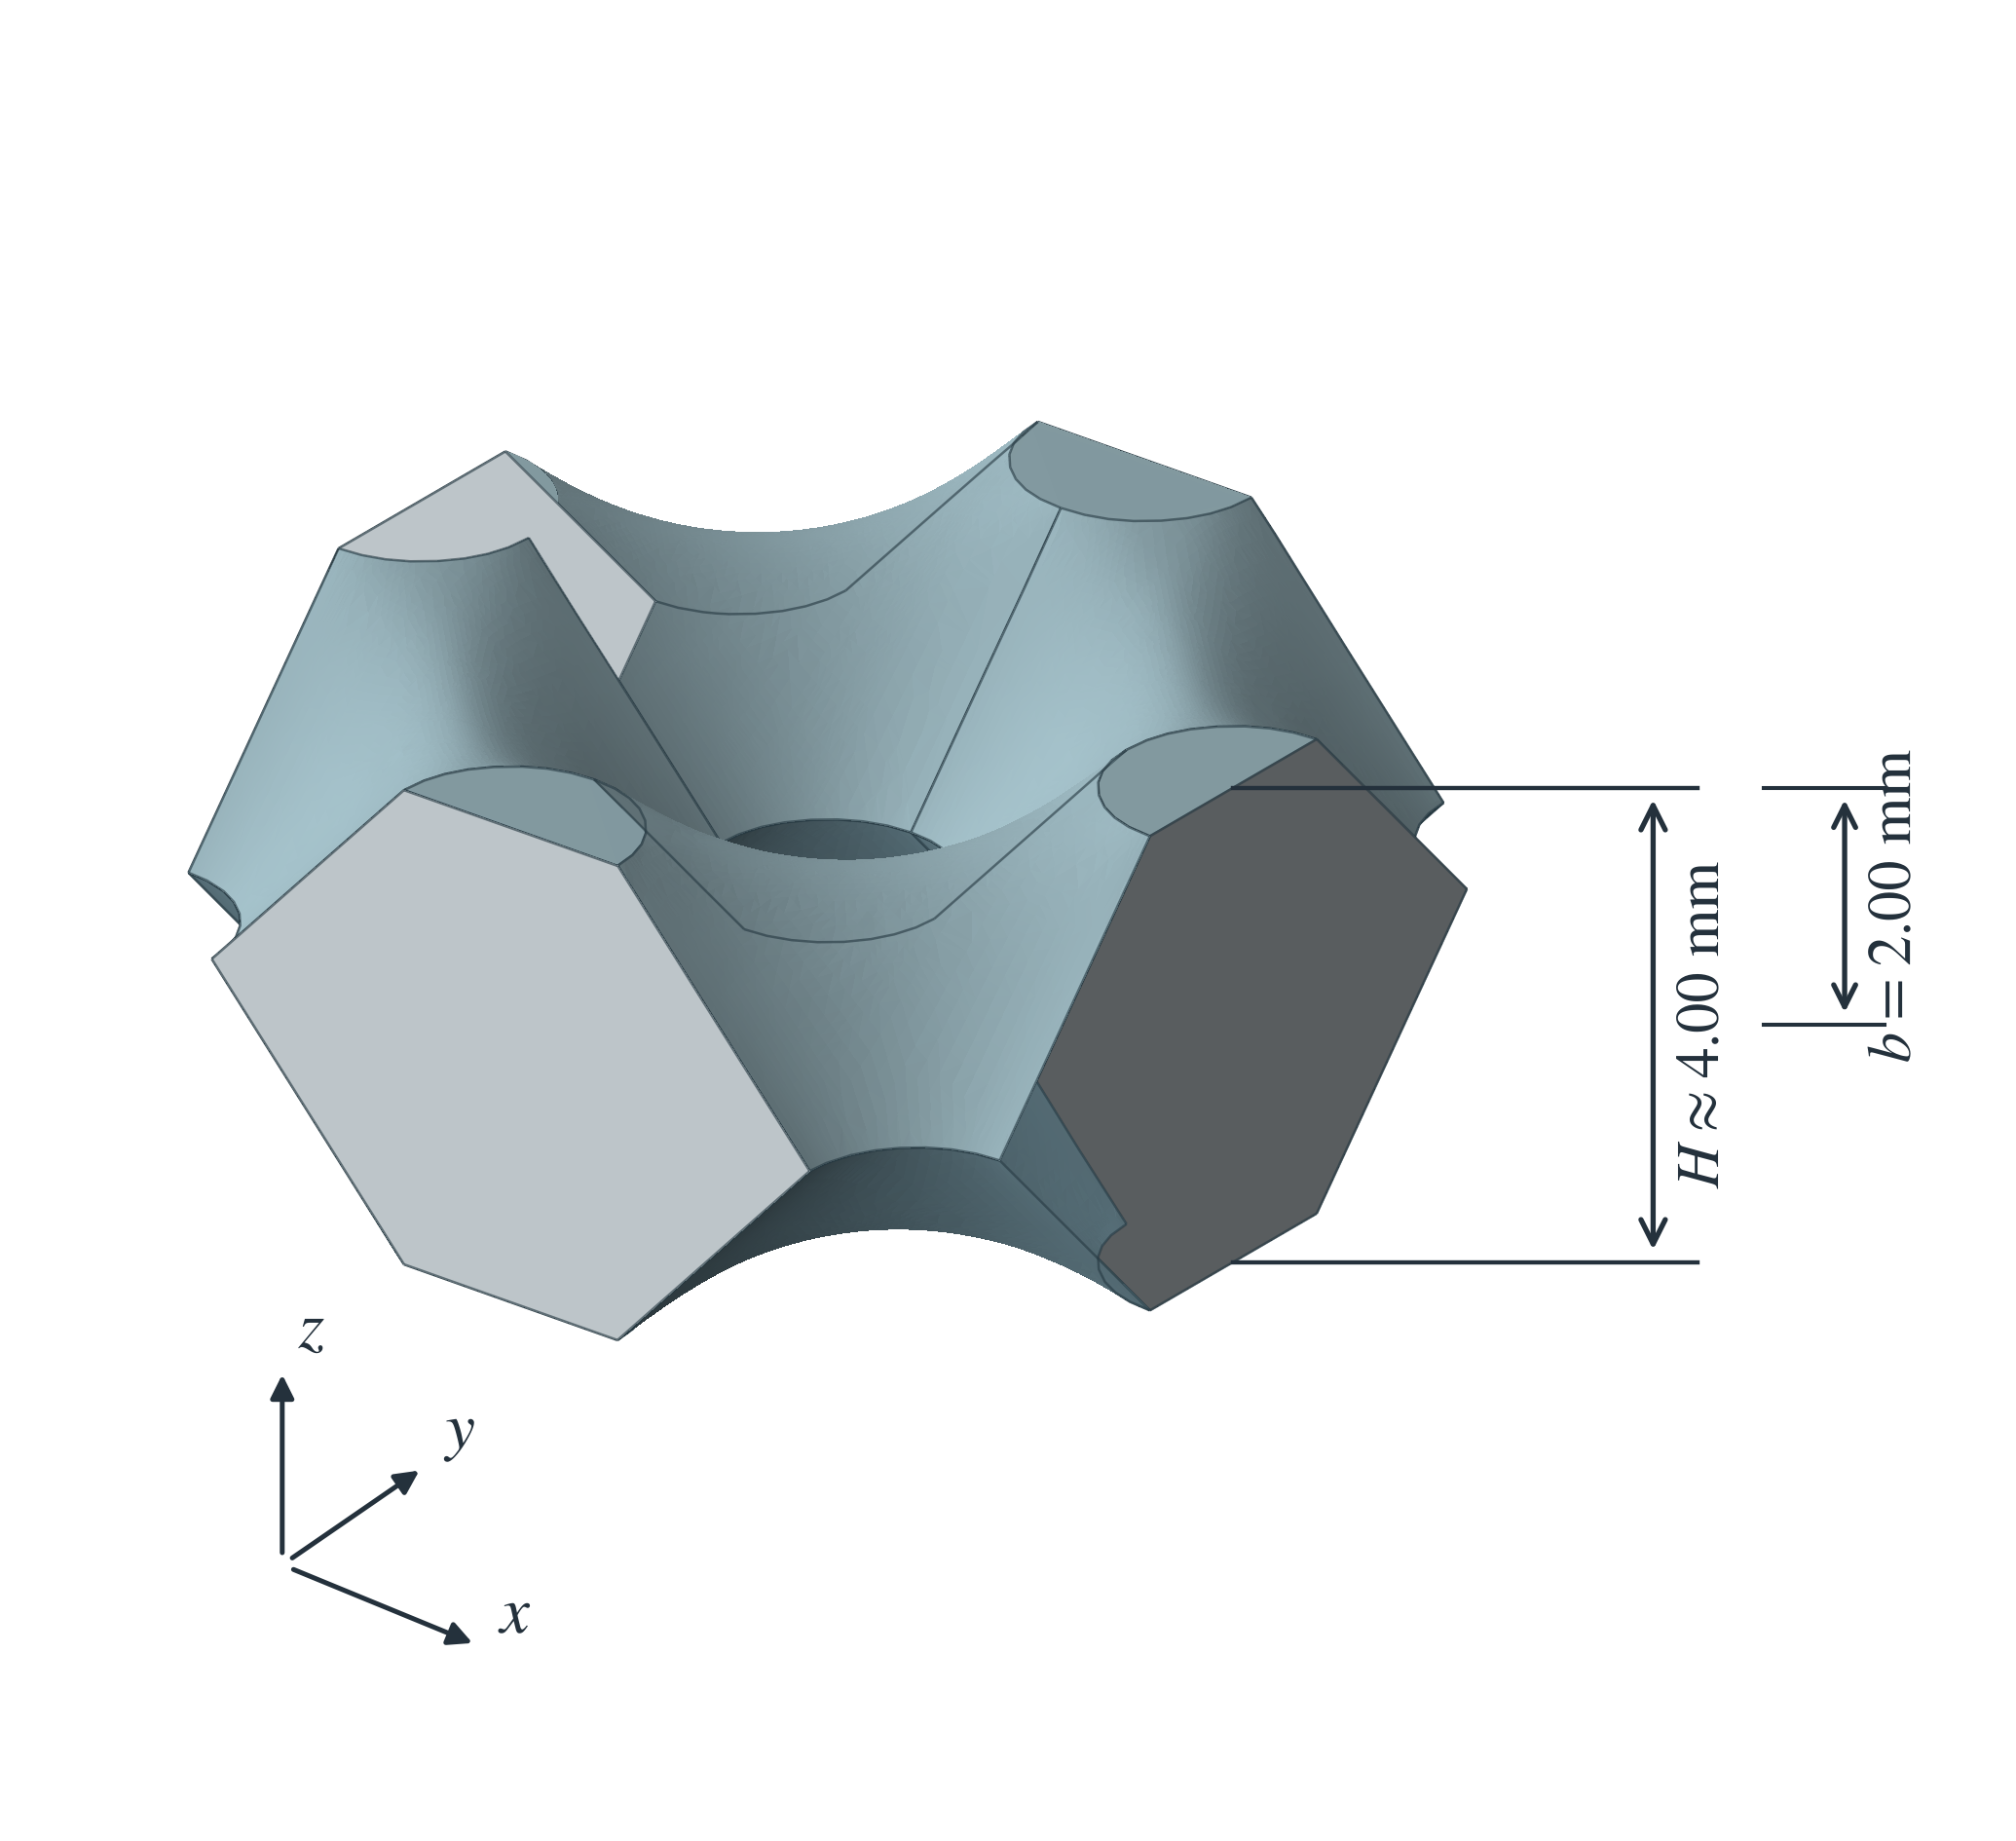
\includegraphics[width=\linewidth]{du_d3_geometry_iso.png}\par
    \small\textbf{(a)} Isometric fluid-domain view
  \end{minipage}\hfill
  \begin{minipage}[t]{0.49\linewidth}
    \centering
    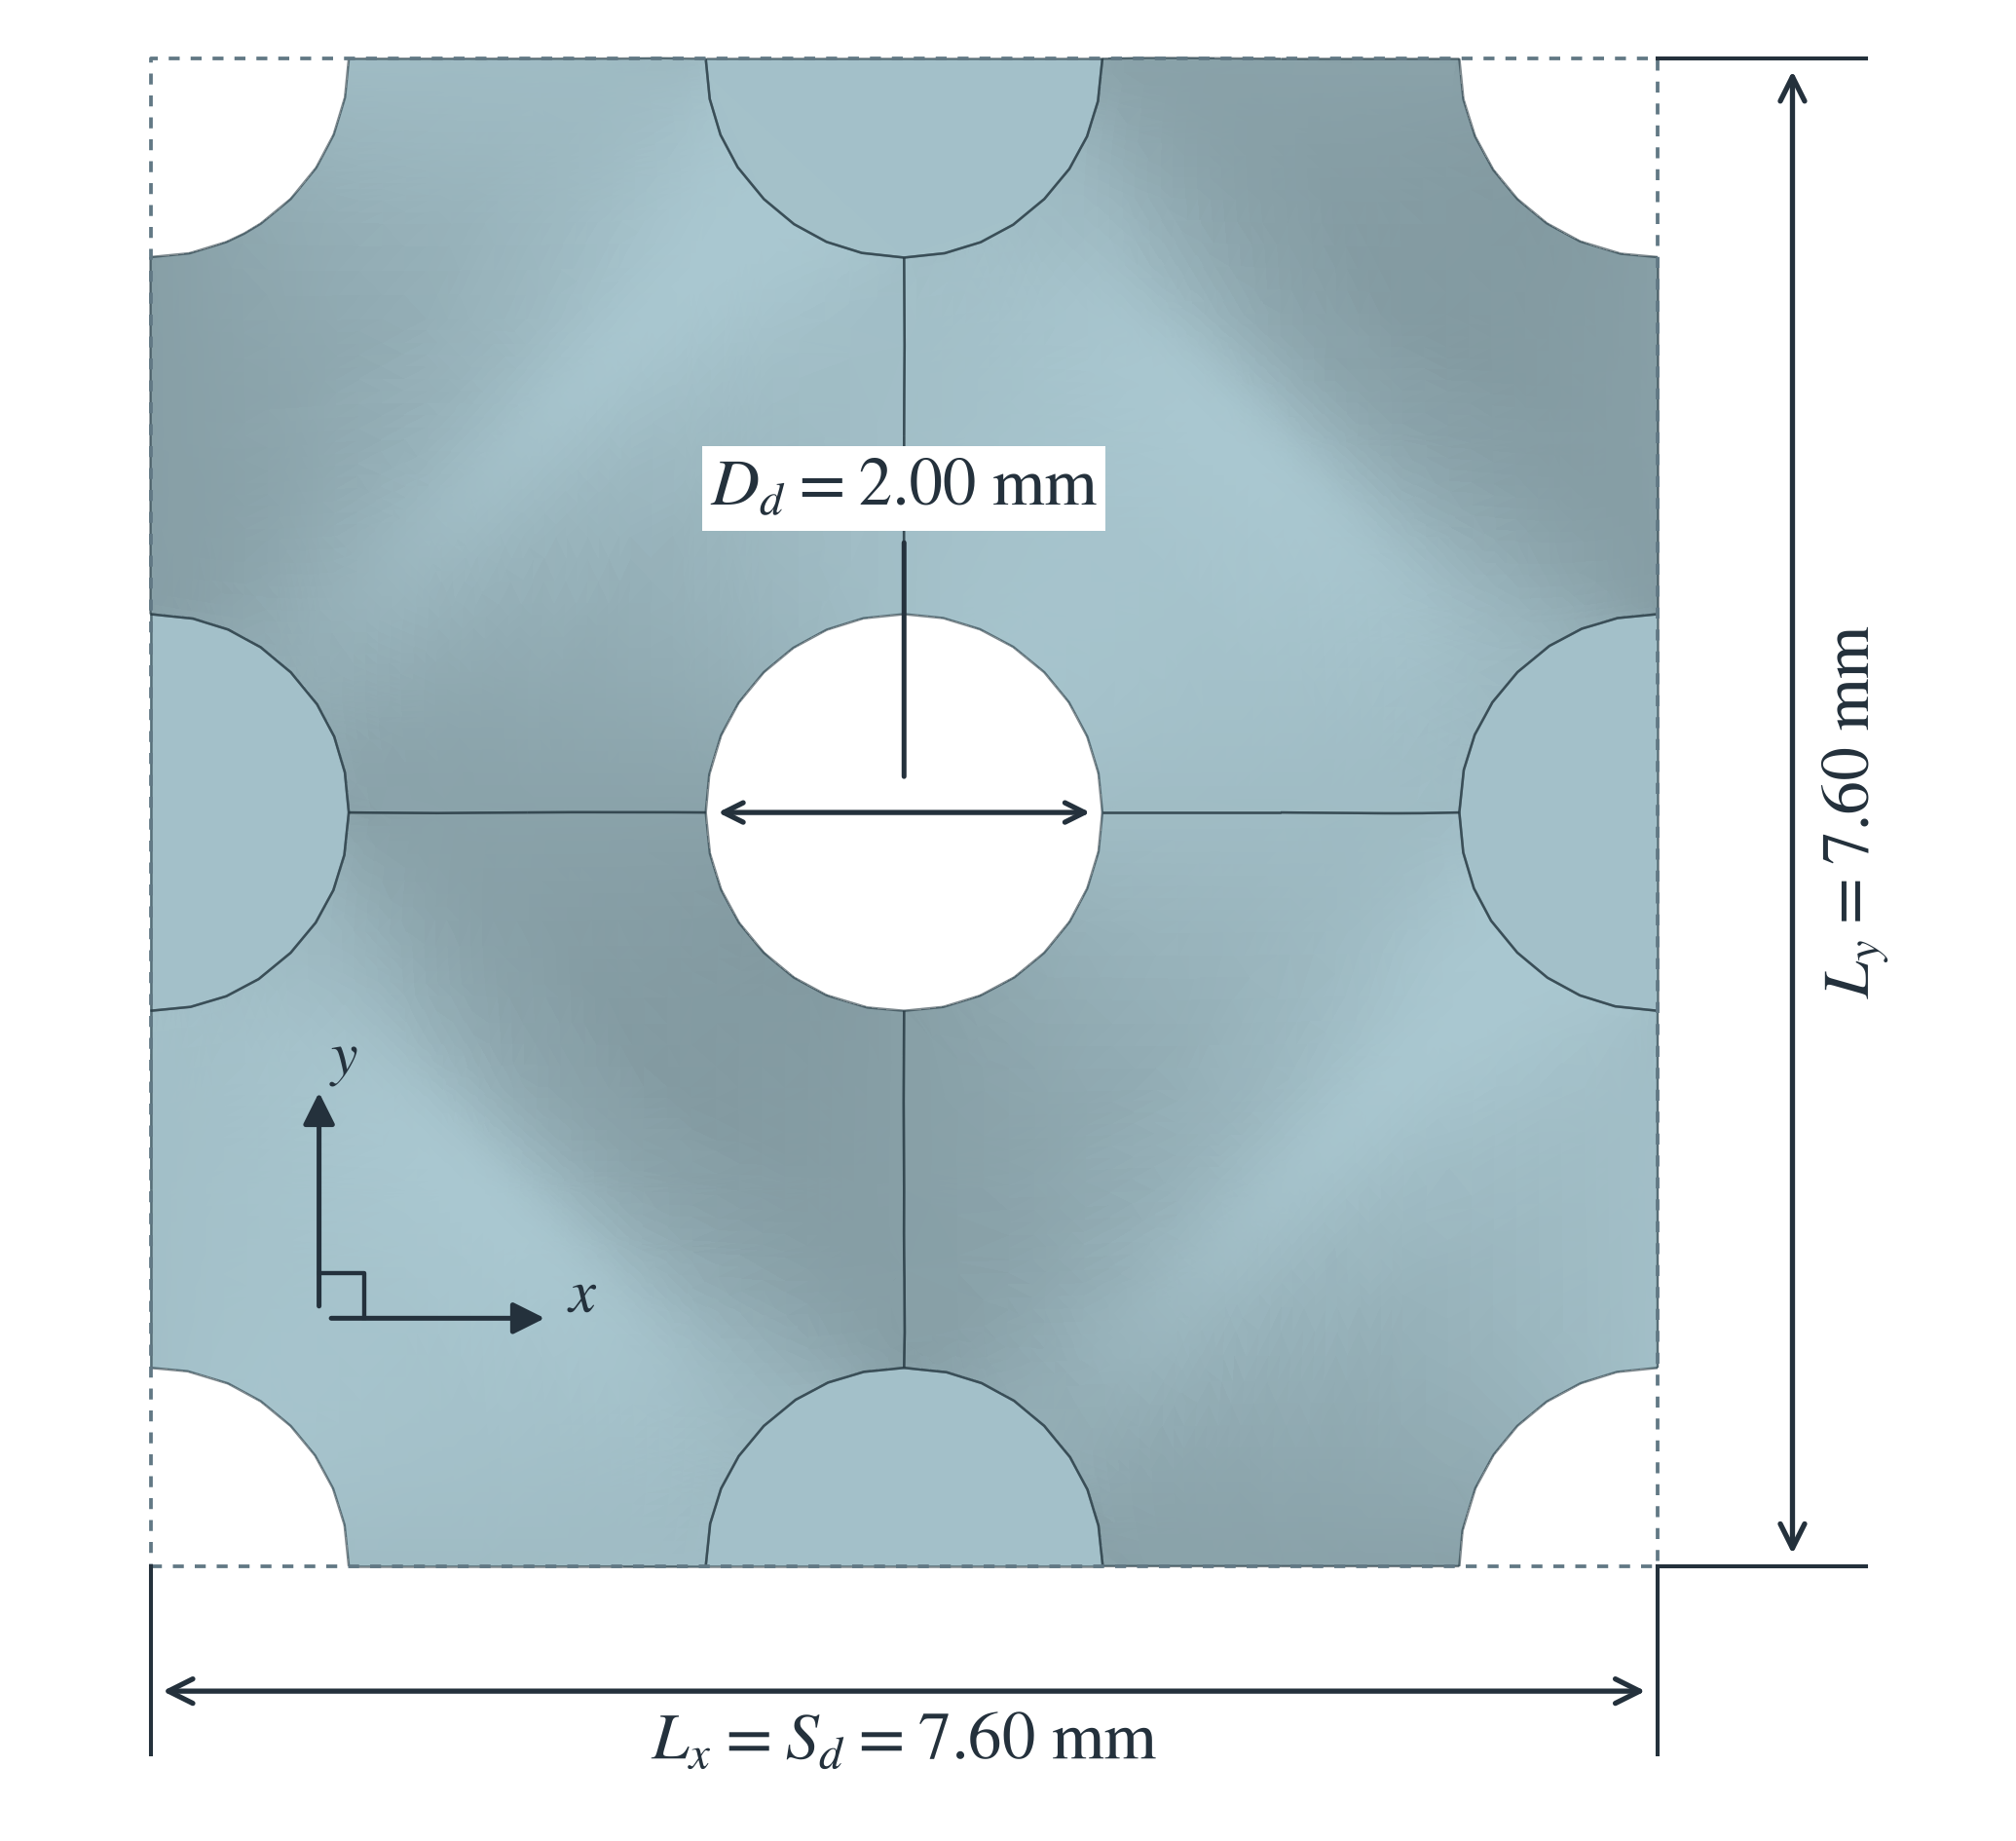
\includegraphics[width=\linewidth]{du_d3_geometry_plan.png}\par
    \small\textbf{(b)} Plan view and repeat dimensions
  \end{minipage}
  \caption{D3 validation unit cell visualised from the supplied CAD fluid domain: (a) isometric view with the nominal pressing depth $b$ and approximate full vertical envelope $H$; (b) plan view with repeat lengths $L_x$, $L_y$ and nominal dimple size $D_d$. Linear dimensions are in millimetres. $S_d$ is the reported dimple pitch. Colours distinguish geometric surfaces and are not solution fields; the central circular footprint is excluded from the fluid.}
  \label{fig:du-d3-geometry}
\end{figure}

\begin{table}[H]
  \centering
  \caption{Dimensions of the D3 benchmark geometry. Reported experimental dimensions follow \citet{du2025}, Table~3; CAD dimensions describe the supplied fluid-domain model. Nominal values are not manufacturing-tolerance or exact surface-matching claims.}
  \label{tab:du-d3-dimensions}
  \small
  \setlength{\tabcolsep}{4pt}
  \renewcommand{\arraystretch}{1.13}
  \begin{tabular}{@{}p{0.32\linewidth}cp{0.12\linewidth}p{0.39\linewidth}@{}}
    \hline
    \textbf{Quantity} & \textbf{Symbol} & \textbf{Value} & \textbf{Definition / source}\\
    \hline
    Unit-cell repeat lengths & $L_x,L_y$ & 7.60~mm & Opposing CAD cut-plane separations in $x$ and $y$.\\
    Dimple pitch & $S_d$ & 7.60~mm & Reported D3 pitch; matches the nominal cell repeat.\\
    Pressing depth & $b$ & 2.00~mm & Reported D3 pressing depth; nominal height from the contact plane to one wall extremum.\\
    Dimple size & $D_d$ & 2.00~mm & Reported D3 dimple size; central contact-footprint diameter in the plan view.\\
    Full vertical fluid envelope & $H$ & $\approx4.00$~mm & Approximate CAD span from $z\approx-2$ to $+2$~mm; not a uniform local channel gap.\\
    Dimple arrangement angle & $\beta$ & $90\degree$ & Reported D3 layout; distinct from the flow-entry angle.\\
    Solid plate thickness & $\delta_p$ & 0.25~mm & Reported experimental plate thickness.\\
    \hline
  \end{tabular}
\end{table}


Figure~\ref{fig:du-d3-mesh} shows the computational mesh of the D3 validation unit cell, comprising 894{,}592 cells.

% Author-supplied D3 mesh image and 894592-cell count, received 2026-10-05.
% The native 440 x 421 image is retained without resampling or content edits.
\begin{figure}[H]
  \centering
  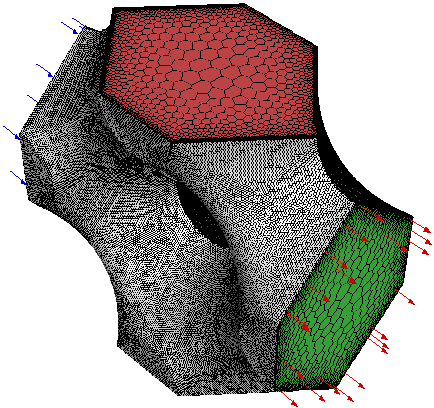
\includegraphics[width=0.38\linewidth]{du_d3_mesh.png}
  \caption{Computational mesh of the D3 validation unit cell, comprising 894{,}592 cells.}
  \label{fig:du-d3-mesh}
\end{figure}


\paragraph{Method-matched quasi-periodic calculation.}
The benchmark retains the steady, single-phase, pressure-based RANS formulation, SST $k$--$\omega$ closure and numerical scheme described in Sections~\ref{sec:numerical_methods} and~\ref{sec:periodic_boundary}. The lateral faces form a translational periodic pair. In the streamwise direction, the velocity inlet and pressure outlet remain separate boundaries: outlet Cartesian velocity components, $k$ and $\omega$ are mapped and scaled onto the inlet between calculation blocks using the existing quasi-periodic loop. The thermal treatment retains a fixed uniform inlet-temperature reset, prescribed isothermal heated walls and no outlet-to-inlet temperature-profile transfer. Hydrodynamic repeatability does not establish thermal periodicity.

The four benchmark points are at $\mathrm{Re}=2089.966$, $4234.524$, $6137.484$ and $6597.217$; the parametric sweeps remain at $\mathrm{Re}=4282$. For each benchmark point, the manuscript's reference-speed relation is
\[
 u=\frac{\mathrm{Re}\,\mu}{\rho D_e}.
\]
Here $D_e$ follows Equation~\eqref{eq:De}, using the D3 cell's own $A_0$, $L$ and both wetted wall areas, not the parametric geometries' 25~mm cell length. The profile-scaling speed $u$, actual inlet-normal bulk speed, net mass flow and mass flux must be distinguished and documented. Du et al. list $D_{\mathrm{hyd}}=4.0$~mm and $D_{\mathrm{eq}}=3.18$~mm and state that hydraulic diameter is used for their Reynolds and Nusselt numbers. 

\paragraph{Heat-transfer reduction and the PA comparison.}
The primary numerical definition remains Equation~\eqref{eq:h_ave}, using both wall heat rates and wetted areas with the fluid-domain mass-average temperature $T_{f,ave}$, followed by Equation~\eqref{eq:Nu}, $\mathrm{Nu}=h_{ave}D_e/\lambda$, where $\lambda$ is water thermal conductivity. Selecting Du's PA series does not change these parametric-study definitions. Du et al. infer their coefficient through exchanger heat-transfer/resistance reduction and evaluate properties at an inlet/outlet bulk-temperature mean. A separately reported PA-equivalent numerical coefficient therefore requires the cell's projected heated area and a stated driving-temperature, property and diameter basis.

\paragraph{Four-point heat-transfer comparison.}
In order of increasing Reynolds number, the present study gives $\mathrm{Nu}=52.75$, $86.38$, $108.14$ and $113.68$, compared with the digitised D3--PA experimental reference values $51.76$, $85.29$, $111.02$ and $116.38$, respectively. Both sets increase monotonically over the four operating points. The signed tabulated difference is defined as
\[
 \delta_{\mathrm{Nu}}=100\,
 \frac{\mathrm{Nu}_{\mathrm{study}}-\mathrm{Nu}_{\mathrm{Du,PA}}}
 {\mathrm{Nu}_{\mathrm{Du,PA}}}\,\%.
\]
The reported signed differences are $+1.92\%$, $+1.28\%$, $-2.60\%$ and $-2.32\%$, respectively. The numerical predictions therefore slightly overestimate the experimental reference at the two lower Reynolds numbers and underestimate it at the two higher Reynolds numbers. Across all four points, the maximum absolute reported difference is $2.60\%$ and the mean absolute reported difference is $2.03\%$.
\begin{table}[H]
\centering
\caption{Four-point comparison of the present quasi-periodic calculation with the provisional digitisation of the open blue D3-PA experimental triangles of \citet{du2025}, Figure~4(b).}
\label{tab:du-validation-comparison}
\small
\renewcommand{\arraystretch}{1.15}
\begin{tabular}{rrrr}
\hline
\textbf{Reported Re} & \textbf{Supplied Du--PA Nu} & \textbf{Present study Nu} & \textbf{$\delta_{\mathrm{Nu}}$ (\%)}\\
\hline
2089.966 & 51.76  & 52.75 & $1.92$\\
4234.524 & 85.29  & 86.38 & $1.28$\\
6137.484 & 111.02 & 108.14 & $-2.60$\\
6597.217 & 116.38 & 113.68 & $-2.32$\\
\hline
\end{tabular}
\end{table}

The D3--PA results of \citet{du2025} are experimentally derived Nusselt numbers and thus provide an independent physical benchmark for validating the present numerical method. Agreement between computed and experimental Nusselt numbers at corresponding Reynolds numbers constitutes validation evidence for the unit-cell heat-transfer predictions, rather than merely agreement between numerical models. The reported four-point agreement therefore supports the method's ability to reproduce both the measured heat-transfer level and its increase with Reynolds number over the sampled D3 range. This validation evidence is specific to the D3 heat-transfer response under the examined conditions.

